\chapter{Background and related work} \label{background}

In this chapter I describe...

\section{Centralized discrete event simulators} \label{centralized-sim}

Event driven simulators typically consist of multiple actors and a scheduler, sometimes referred to as the event queue. %todo ref(s)
The scheduler is the driver of the simulation, its operation fairly straightforward: execute the next event, insert any new events at an appropriate place in the queue, launch the next event.
The relatively simple nature of the scheduler makes it so that it can usually be implemented in relatively few lines of code.
For the sequential simulator, RotorSim\cite{brode-roger_nibriviarotorsim_2020} described in \S \ref{rotorsim}, the loop and event processing code takes up around 30 lines of python.

% not happy with this paragraph structure
Large simulation models can generate millions or billions of events through their lifetime, causing the queue to continuously hold thousands or more events at a time, see the results section \S\ref{results} for more details.
In addition, since events are typically fast to process, the queue is also continuously being accessed and modified and can easily become a bottleneck.
The large size and frequent access of the queue, force careful consideration of the data structures used to implement the queue/

The queue has to support two operations: retrieving the smallest element currently in the queue, and inserting new events.
This naturally leads to using a min-heap, allowing for $O\left(\log n\right)$ insertion and removal of the smallest element.
Although there exists slightly faster "monotonic heaps", such as the Ladder Queue \cite{tang_ladder_2005}, that are able to further either the complexity or the constant factor, they are usually complex to implement and tune \cite{furfaro_adaptive_2018}, and don't have available efficient implementations.
Standard heaps however are common enough that most every language has a well-optimized implementation, often making them easier to use.

Fundamentally, these simulations are centralized: the scheduler drives the model forward.
Some parallelization is possible if many events are scheduled at the same virtual time and the actors are able to deal with that.
Even if the simulation has many events executing in parallel, we run into issues when they try to schedule new events: the scheduler needs to manage multiple new events being enqueued concurrently.
In my experience, the overhead of managing these concurrent operations results in worse performance overall.

\paragraph{Preservation of causality}

In order for a simulation to be correct, it is essential that before any event is processed, all past events it depends on have taken effect.
The dependency on these prior events may be obvious: a packet needs to arrive at a router before it can be sent from said router, or not: in order to know where in the queue to place the arriving packet, it is necessary to know \emph{every} other arriving packet, even if it is from a different source and to a different destination, a previous packet may fill up the router's available memory.

The centralized simulator ensures causality by processing events in absolute time order: by the time any event is executed, all events in its past have fully completed.
Events happening simultaneously are typically assumed to not affect each other and can therefore happen in any order.

\paragraph{Guarantee of progress}
This simulator will always make progress as long as there is another event to process, trivially allowing it to keep making progress until there is none left.



\section{Parallel discrete event simulators} \label{pdes}

The main difficulty in making event simulators parallel lies in guaranteeing causality and progress.
It is often easy to guarantee one without the other: without preserving causality, we can process events out of order, and without a need for progress, we are free to advance until it becomes too difficult, and stop then.
Clearly, neither of these solutions are satisfying.

I will describe first the opportunities for concurrency in distributed simulations, then focus on the issues that are raised by needing to make progress.

\subsection{Causality preservation} \label{causality}

%TODO make diagram
\begin{figure}
    \centering
    \begin{subfigure}[t]{0.45\textwidth}
        \centering
        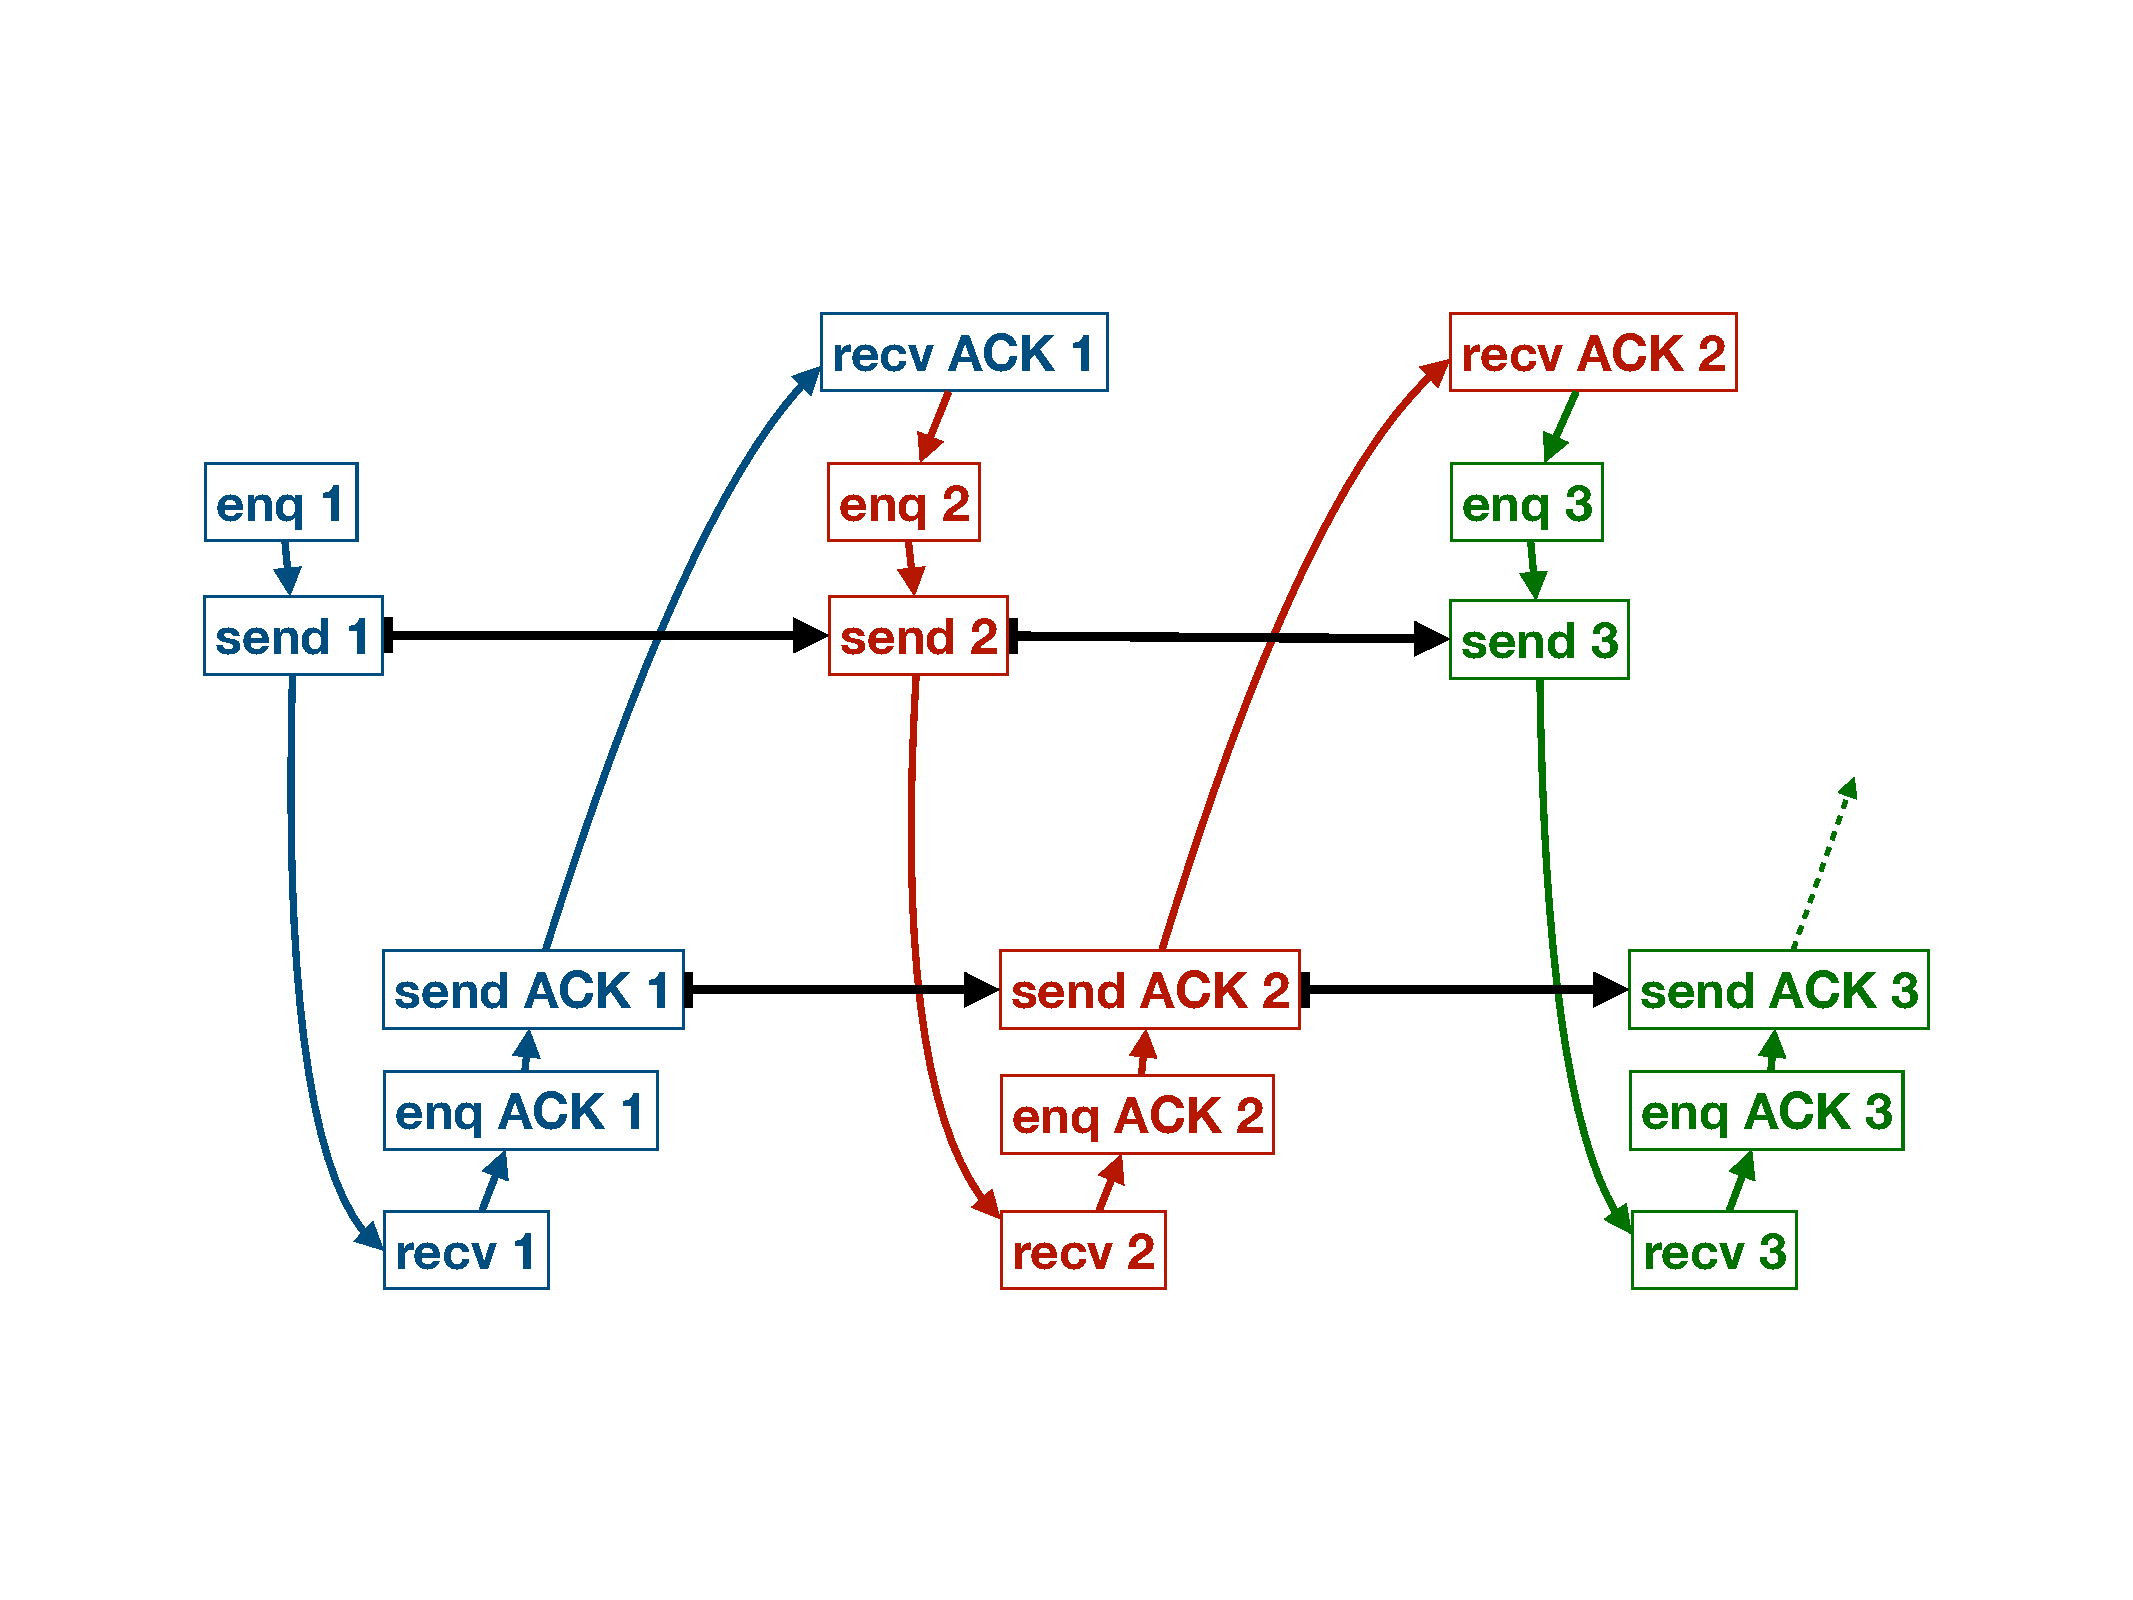
\includegraphics[width=\textwidth]{causality-single}
        \caption{
            This series of events has no opportunity for concurrency: every event directly depends on the previous one.
        }
        \label{causality-graph-seq:fig}
    \end{subfigure}
    \begin{subfigure}[t]{0.45\textwidth}
        \centering
        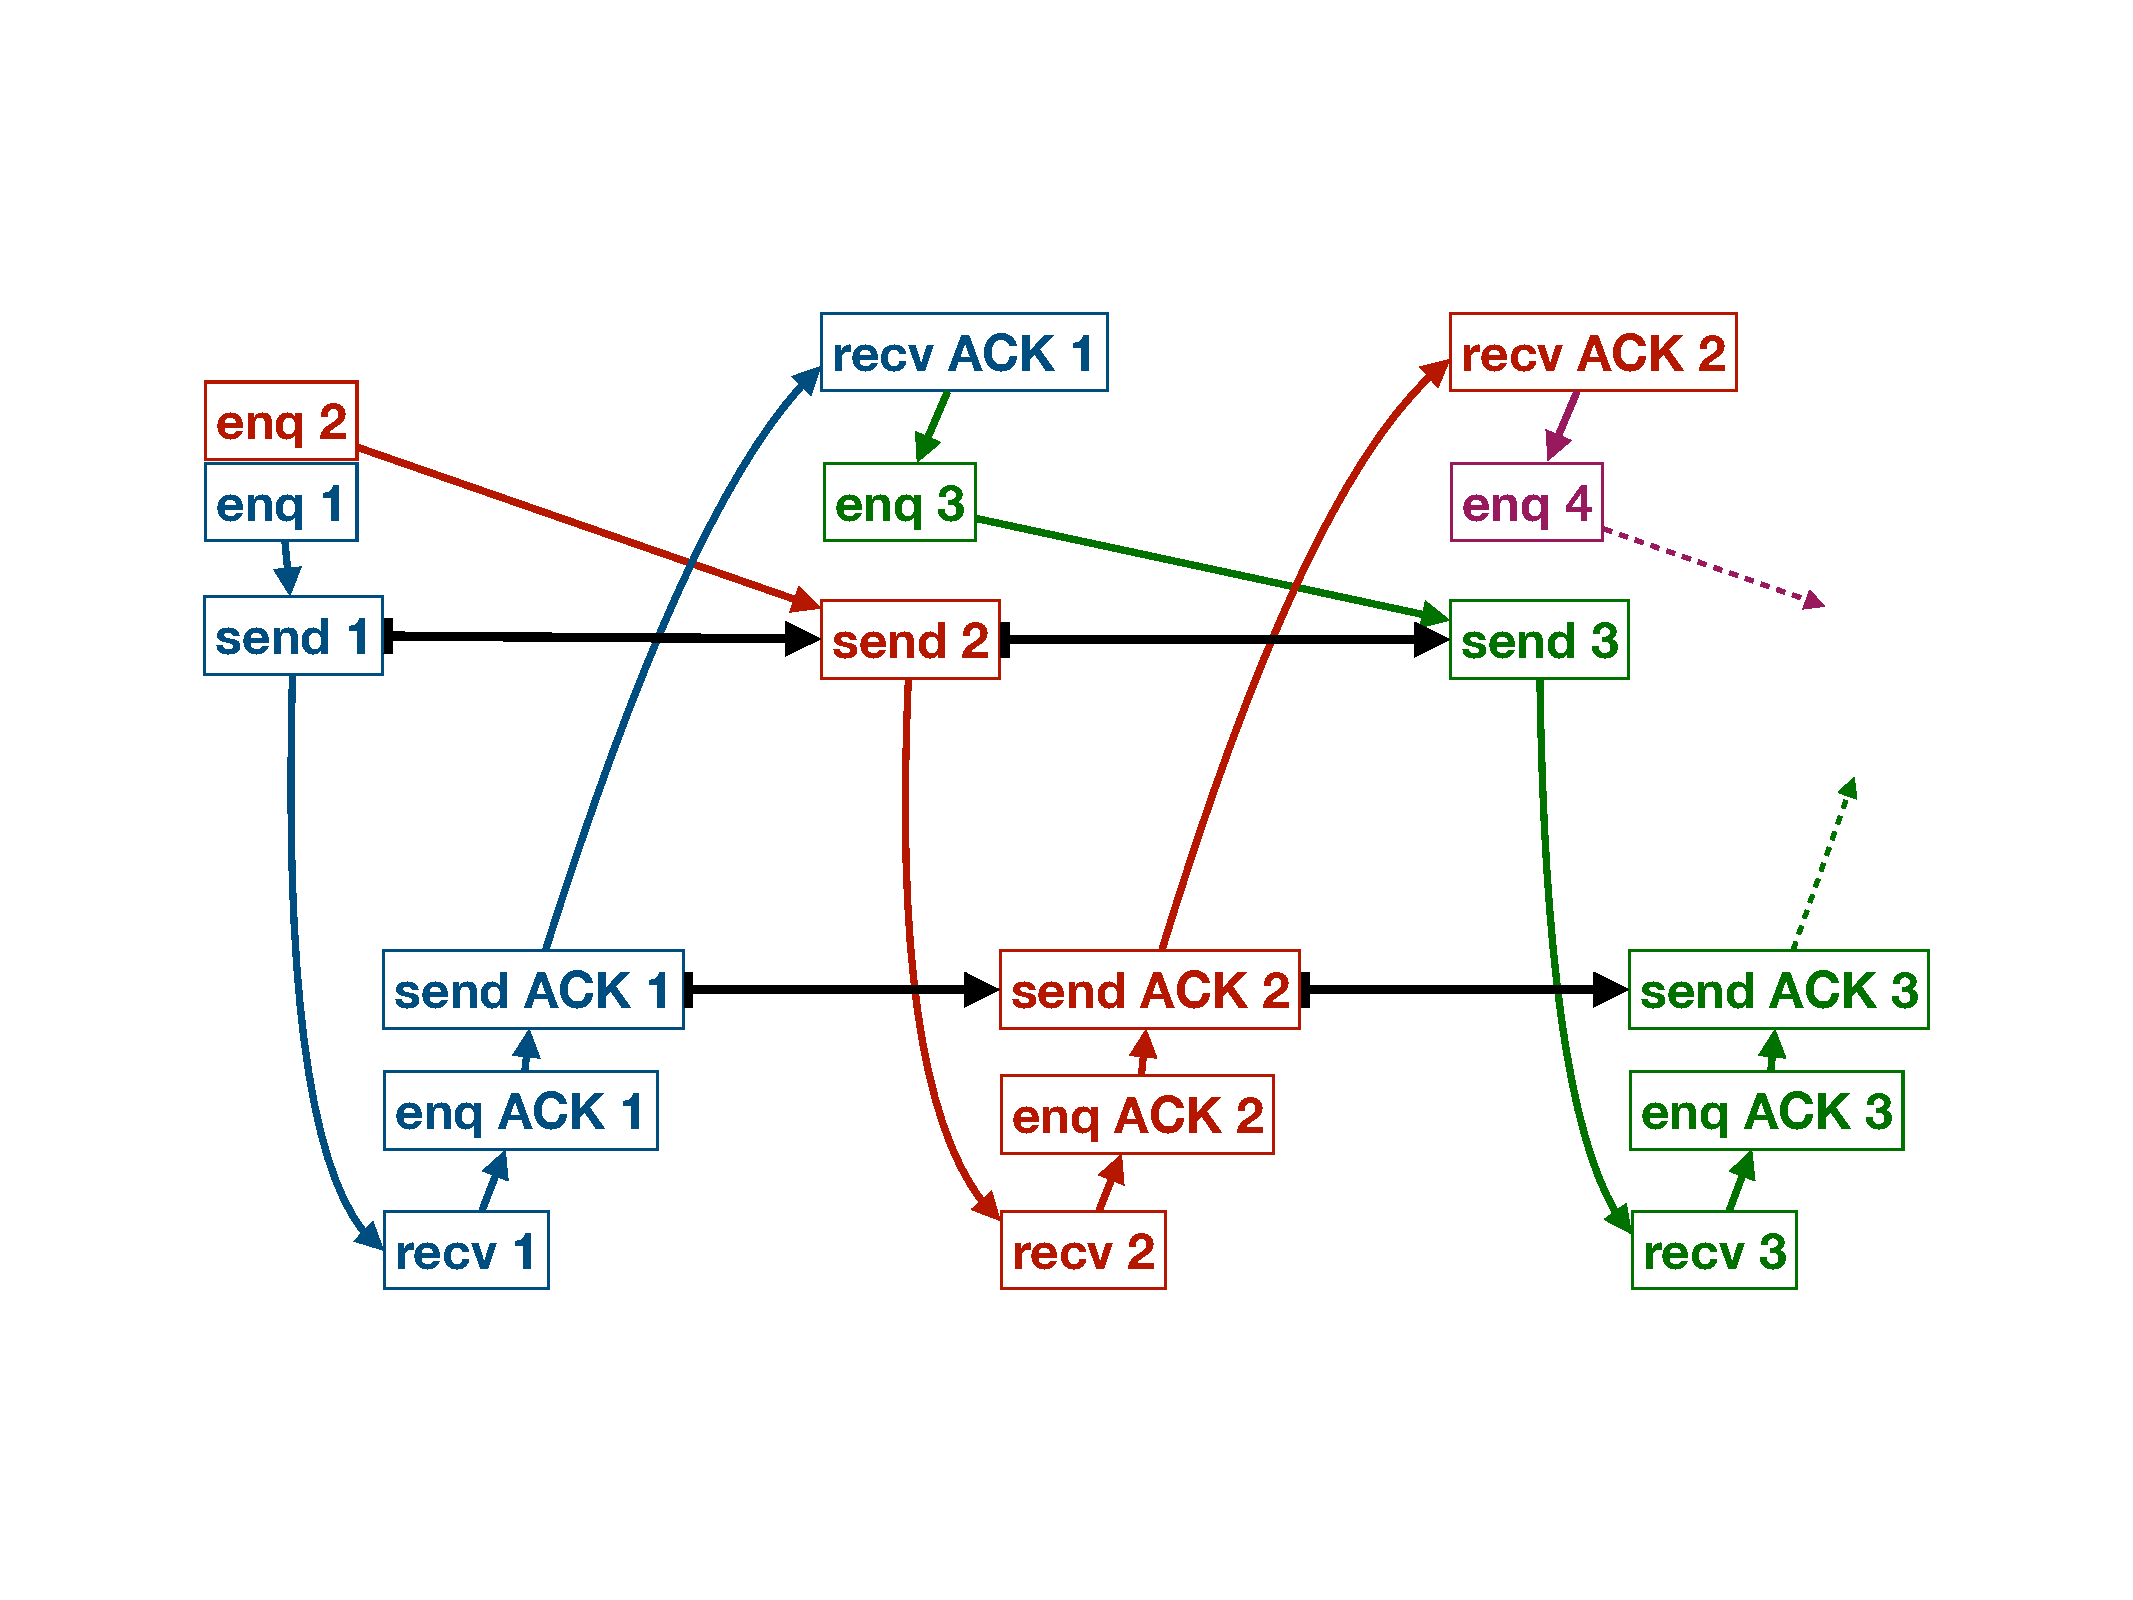
\includegraphics[width=\textwidth]{causality-concurrent}
        \caption{
            However, when the congestion window is larger, some events are independent from each other, for example \code{recv 1} and \code{send 2}.
        }
        \label{causality-graph-seq:fig}
    \end{subfigure}
    \caption{
        These two causality graphs are very similar, however, one permits concurrency and the other does not.
        Each graph corresponds to a sketch of a TCP exchange with a congestion window of 1 or 2.
        The arrows represent a direct dependency between two events, the black arrows between successive sends correspond to how long it takes to transmit a single packet.
        Every send implicitly depends on previous sends.
    }
    \label{causality-graph:fig}
\end{figure}

To better understand the opportunity, or lack thereof, for parallelization, it is necessary to better understand what causality requirements are imposed by the model.
A useful tool for this job is a causality graph.
A causality graph consists of a node for each event in the simulation, and a directed edge between from a dependency to the future event.
Any topological sort of the resulting graph is a valid execution order of the events.
Since the direction of the graph is always to the future, sorting the events by time is trivially correct.
This is the approach taken by the centralized simulator.

If a pair of events are direct ancestors/descendants of each other, i.e. there is a direct line going from one to the other, then there is a dependence between each other and they may not be executed simultaneously.
Conversely, if there is no direct connection between two events, they may be executed simultaneously.
This does not prevent events from sharing a common ancestor or descendant.

These events that are neither ancestor nor descendants are essentially independent of the current event, they can happen before, or after, or simultaneously, it will not affect the correctness of the simulation.
This is very similar to events outside the light-cone in physics: events outside the light cone cannot have a causal relationship with the current point.
The correctness guarantee can therefore be reduced to knowing whether the next event to process has had all of its ancestors have been processed, i.e. it is safe.

From an actor-centric point of view, this guarantee comes down to knowing if the next event available to process is in fact the next event.
% TODO

An old algorithm, described as early as 1986\cite{misra_distributed_1986}, TODO...

\subsection{Null-message passing} \label{null-messages}

Unfortunately, waiting on each of our neighbours to send us an event is prone to deadlocking.
For example, in a network simulation where there are no packets to send, actors will not be sending any events to each other.
Every actor will therefore be waiting for its neighbours, 

\subsection{Other approaches}

Although the process described above is what I will be implementing in this thesis, other options exists for parallel discrete-event simulators.
Two are worth highlighting, both sacrifice accuracy in some way in order to obtain better performance.
The difference between the two approaches comes down to wether that accuracy error gets resolved or no.

\paragraph{Optimistic scheduling} \label{optimistic-scheduling}
It is also possible to allow actors to process events as fast as they can, possibly resulting in causality violations.
In order to maintain correctness, the simulation needs to have a cancellation mechanism, some use anti-events \cite{} or checkpointing \cite{}. %todo cite
This hopeful approach is the source of its name.

The cost of optimistic scheduling comes from the overhead necessary to allow for rollbacks, and the execution of these rollbacks.
\emph{TimeWarp} \cite{} is a popular example of an optimistic scheduling algorithm.

Trying and rolling back is a common technique in computer engineering.
Databases use optimistic concurrency control instead of locks to rollback transactions in case of a conflict \cite{dragojevic_no_2015}.
CPUs are continuously predicting the next instruction to allow for higher speeds, but also need a cancelling mechanism if the prediction turns out incorrect.

Although correct, I have not explored this strategy out of a belief that it requires too much additional book-keeping to be useful.
This assumption has proven to be correct, on similar models, my simulator performs better than state of the art optimistic simulators.

However, optimistic simulators are able to make progress in models that the null-message passing algorithm cannot.
A null-message passing strategy relies on there being latency between actors, allowing them to make progress with respect to each other.
However, if the model asks for actors that may send each other events with no intervening delay, conservative simulators can get stuck: progress cannot be made if neither actor knows whether to expect an event from the other.
% mention rarely used small latency?
There are often ways to restructure the model in order to eliminate this situation, but this type of scenario is where optimistic strategies shine.

\paragraph{Loss of accuracy}
Another strategy could be to let execute events in the wrong order, possible yielding incorrect results.
Indeed, in an accurate simulator, incorrect results can result from an incorrect model or an incorrect simulator.
However, when giving up accuracy, the model may be correct, and properly implemented, but the results may still be off due to an unlucky run or a simulator bias.
Fundamentally, this makes trusting the results of the simulator harder.
In this thesis, correctness is an important design goal since it eliminates a source of errors, and I thus do not explore this strategy.
